% =====================================================================
%  QM composite for metabolic reaction free energies — progress deck
%  Compile with:  lualatex thermo_progress.tex   (twice)
% =====================================================================
\documentclass[aspectratio=169,11pt]{beamer}

\usetheme{metropolis}
\metroset{block=fill, sectionpage=progressbar, numbering=fraction}

\usepackage{booktabs}
\usepackage{amsmath}
\usepackage{siunitx}
\usepackage{graphicx}
\usepackage{xcolor}

% ---- palette ---------------------------------------------------------
\definecolor{accent}{HTML}{2A6F97}     % deep teal-blue
\definecolor{good}{HTML}{2E8B57}       % green  (works)
\definecolor{bad}{HTML}{C0392B}        % red    (fails)
\definecolor{muted}{HTML}{6C757D}
\definecolor{darkbg}{HTML}{22303C}
\setbeamercolor{normal text}{fg=black!88}
\setbeamercolor{alerted text}{fg=accent}
\setbeamercolor{frametitle}{bg=darkbg,fg=white}
\setbeamercolor{progress bar}{fg=accent,bg=accent!25}

% ---- helpers ---------------------------------------------------------
\newcommand{\dg}{\ensuremath{\Delta_r G'^{\circ}}}
\newcommand{\kj}{\,kJ/mol}
\newcommand{\yes}{\textcolor{good}{\textbf{\checkmark}}}
\newcommand{\no}{\textcolor{bad}{\textbf{\ding{55}}}}
\usepackage{pifont}
\newcommand{\win}[1]{\textcolor{good}{\textbf{#1}}}
\newcommand{\lose}[1]{\textcolor{bad}{#1}}

\title{Can Quantum Chemistry Referee Metabolic \dg?}
\subtitle{A QM/ML composite vs.\ dGPredictor on TECRDB disagreements}
\author{ModelSEED thermodynamics project}
\date{Progress summary — August 2026}

% =====================================================================
\begin{document}

\maketitle

% ---------------------------------------------------------------------
\begin{frame}{The question, and the short answer}
  \begin{block}{Motivating question}
    ModelSEED's retrained \textbf{dGPredictor} disagrees with experiment
    (TECRDB) on a set of reactions by 16--100\kj. Can a
    \textbf{parameter-free quantum-mechanical} method \emph{adjudicate} those
    disagreements — from physics, sharing none of dGPredictor's
    group-contribution basis?
  \end{block}
  \begin{columns}[T]
    \column{0.5\textwidth}
      \textbf{Short answer: no — and it need not.}
      \begin{itemize}
        \item The data-driven \textbf{eQuilibrator} already matches
              experiment to within its noise (MAE \win{3.6}\kj, exp.\ sd 6.2).
        \item Our QM composite sits at \lose{38.3}\kj\ — it cannot
              referee a 100\kj\ gap when its own error is $\sim$38.
      \end{itemize}
    \column{0.5\textwidth}
      \textbf{What QM \emph{can} defensibly do}
      \begin{itemize}
        \item On glutathione redox its \emph{magnitude} ($\sim$36\kj)
              independently excludes dGPredictor's $\sim$103 —
        \item from a method trained on \textbf{zero} thermodynamic data.
        \item That corroboration, not a competitive MAE, is the usable result.
      \end{itemize}
  \end{columns}
\end{frame}

% =====================================================================
\section{Methodology}
% =====================================================================

\begin{frame}{The composite — what is computed}
  For every metabolite we build an aqueous standard Gibbs energy, then combine
  species into reactions and transform to physiological conditions.
  \[
    \boxed{\,G_{\text{aq}} \;=\;
      \underbrace{E_{\text{MLIP}}^{\text{gas}}}_{\text{UMA / MACE-POLAR}}
      \;+\;
      \underbrace{\Delta G_{\text{solv}}^{\text{ALPB}}}_{\text{xtb GFN2}}
      \;+\;
      \underbrace{G_{\text{RRHO}}}_{\text{quasi-RRHO thermal}}\,}
  \]
  \begin{columns}[T]
    \column{0.54\textwidth}
    \begin{enumerate}
      \item Enumerate conformers; optimise \textbf{in ALPB water}.
      \item Single-point gas energy on that same geometry
            (electronic + solvation share one structure).
      \item One Hessian per compound $\rightarrow$ thermal correction.
      \item \textbf{Boltzmann-average} over conformers.
    \end{enumerate}
    \column{0.46\textwidth}
    \begin{enumerate}\setcounter{enumi}{4}
      \item Combine into \dg\ per reaction.
      \item \textbf{Alberty} Legendre transform to the measured pH
            $+$ extended \textbf{Debye--H\"uckel} (ionic strength).
    \end{enumerate}
    \vspace{0.4em}
    \begin{alertblock}{Key discipline}
      Corrections are calibrated \emph{only} on external experimental
      \textbf{pKa} values — never on the reactions being scored.
    \end{alertblock}
  \end{columns}
\end{frame}

\begin{frame}{Why this design, and what it is \emph{not}}
  \begin{columns}[T]
    \column{0.5\textwidth}
      \textbf{The error budget (per reaction)}\\[0.3em]
      A solvated polyanion computed absolutely carries continuum-solvation
      error on ions ($\sim$15\kj/species), plus conformational, RRHO and
      electronic error. Four species, uncorrelated:
      \[
        \sqrt{4}\times 15 \;\approx\; 30\kj
      \]
      Measured scatter: 42 (130 rxns), 34 (cleanest subset).
      The gap to the 3--8\kj\ ``useful'' target is \textbf{structural}, not a
      tuning problem — and reproduces Jinich \emph{et al.}, \emph{Sci.\ Rep.}\ 2014.
    \column{0.5\textwidth}
      \textbf{The bottleneck is \emph{not} the electronic method}\\[0.3em]
      \begin{itemize}
        \item Substituting real DFT (r2SCAN-3c) for the MLIP at fixed
              geometry made it \lose{worse} (14.9 $\to$ 17.3).
        \item UMA vs.\ MACE-POLAR agree at $r=0.98$ (spread 7 vs.\ error 40).
        \item Solvation is the driver: continuum models
              \textbf{under-solvate multiply-charged anions}
              ($\sim$30\kj\ per reaction).
      \end{itemize}
      \vspace{0.3em}
      $\Rightarrow$ every phosphate/polyanion pays the same structural tax.
  \end{columns}
\end{frame}

% =====================================================================
\section{Implementation}
% =====================================================================

\begin{frame}{Pipeline — data in, \dg\ out}
  \small
  Nothing is hard-coded to a reaction set: reactions, metabolites and
  measurement conditions are all read from data.
  \begin{center}
  \begin{tabular}{@{}clll@{}}
    \toprule
    \# & stage & where & what \\
    \midrule
    1 & \texttt{build\_inputs}        & CPU          & ModelSEED reactions/metabolites $\to$ JSON \\
    2 & \texttt{microspecies}         & CPU          & audit SMILES for protonation / hydration state \\
    3--4 & \texttt{build\_ensembles}  & CPU (xtb)    & ETKDG embed $\to$ GFN2 opt (ALPB) $\to$ Hessian \\
    5 & \texttt{run\_uma\_ensemble}   & \textbf{multi-GPU} & UMA gas energy per conformer, Boltzmann avg. \\
    6 & \texttt{analyze\_pka}         & CPU+GPU      & anion-solvation calibration (one-time, reusable) \\
    7 & \texttt{final\_model}         & CPU          & score reactions $\to$ \texttt{perreaction\_dG.csv} \\
    8 & \texttt{plot\_comparison}     & CPU          & figures \\
    \bottomrule
  \end{tabular}
  \end{center}
  \begin{columns}[T]
    \column{0.5\textwidth}
      \textbf{Compute} (23 metabolites, 605 conformers):
      conformer ensembles $\sim$35 min (dominates, $\sim$2 core-h/metabolite);
      UMA scoring $\sim$3.5 min on 8$\times$V100.
    \column{0.5\textwidth}
      \textbf{Scales linearly}: $\sim$1000 metabolites $\approx$ 2000 core-hours
      $\approx$ 25 h on 80 cores; GPU time negligible.
  \end{columns}
\end{frame}

\begin{frame}{Two engineering checks that matter}
  \begin{columns}[T]
    \column{0.5\textwidth}
      \textbf{Geometry sufficiency}\\[0.2em]
      r2SCAN-3c geometry vs.\ expensive wB97M-V/def2-TZVPD single point:
      all $|\Delta E| < 2\kj$ and RMSD $\le 0.017$\,\AA.
      \emph{Cheap geometries are good enough} — no expensive re-optimisation.
      \begin{center}
        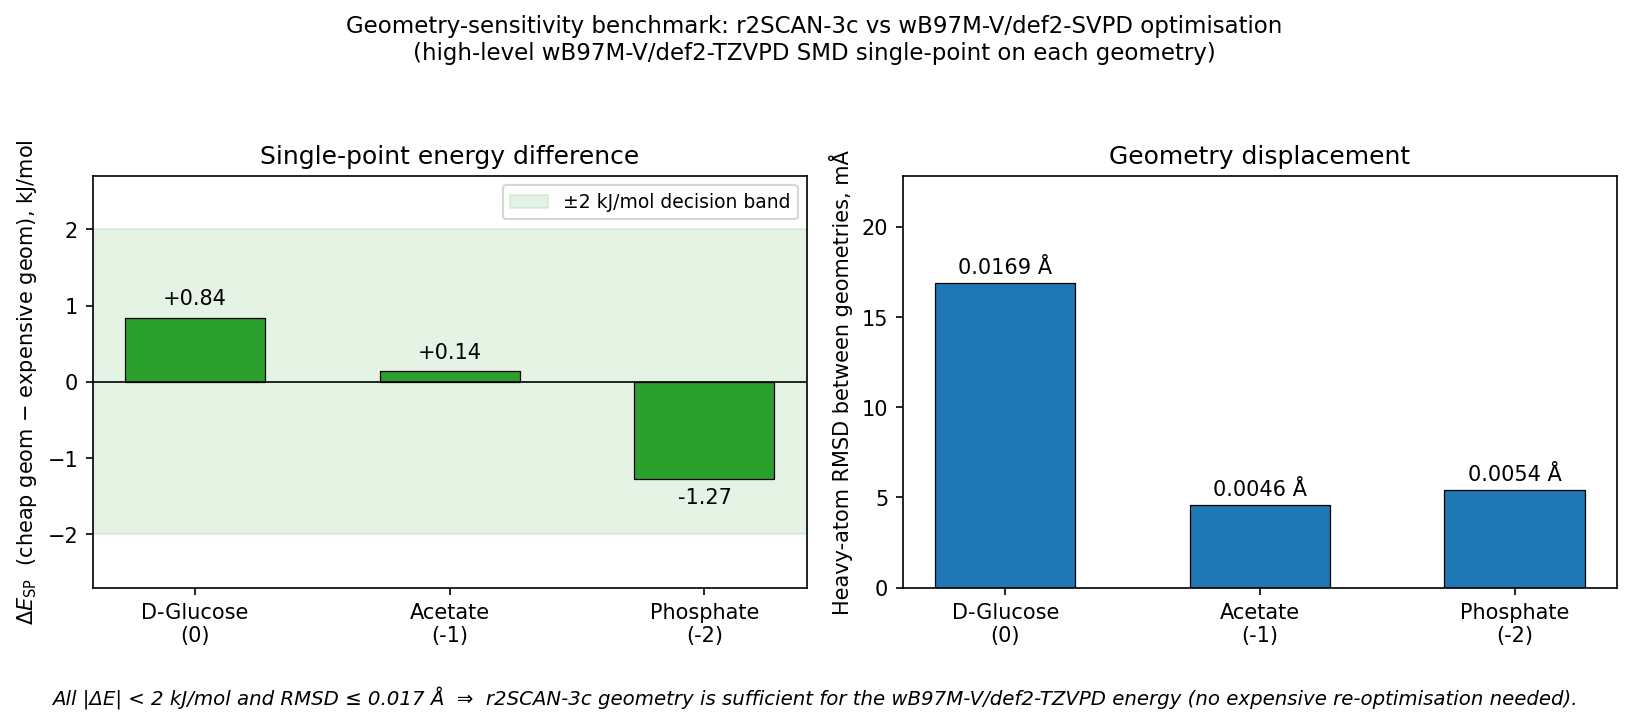
\includegraphics[width=\linewidth]{figures/qm_geometry_sensitivity.png}
      \end{center}
    \column{0.5\textwidth}
      \textbf{The Alberty transform passes independently}
      \begin{itemize}\small
        \item ATP hydrolysis $-35.3$ vs.\ published $-32.5$.
        \item Debye--H\"uckel scales as $\Delta(z^2)$ exactly $1{:}4{:}9{:}16$.
        \item pH slope exact.
      \end{itemize}
      \vspace{0.3em}
      \textbf{Bugs found \& fixed} (each moved the answer):
      \begin{itemize}\small
        \item Missing standard-state term $RT\ln(24.46)=7.93\kj$/species
              (hid in $\Delta n\!=\!0$ isomerisations).
        \item Quality screen rejected acetic acid — now screens on imaginary-mode
              \emph{magnitude} (50\,cm$^{-1}$), not presence.
      \end{itemize}
  \end{columns}
\end{frame}

% =====================================================================
\section{Results}
% =====================================================================

\begin{frame}{Headline — the ten disagreement reactions}
  \begin{columns}[T]
    \column{0.46\textwidth}
      \begin{center}
      \begin{tabular}{@{}lr@{}}
        \toprule
        method & MAE vs.\ TECRDB \\
        \midrule
        \win{eQuilibrator}      & \win{3.6}\ \tiny(exp.\ sd 6.2) \\
        predict zero            & 10.5 \\
        QM, isodesmic (best)    & 24.6 \\
        GroupContribution       & 35.4 \\
        \textbf{QM composite}   & \textbf{38.3} \\
        \lose{dGPredictor}      & \lose{61.2} \\
        \bottomrule
      \end{tabular}
      \end{center}
    \column{0.54\textwidth}
      \begin{alertblock}{The ten are already solved}
        eQuilibrator agrees with TECRDB on \emph{exactly} the reactions
        dGPredictor fails. So the adjudication verdict is
        ``\textbf{dGPredictor is the outlier}'' — and it needs no quantum chemistry.
      \end{alertblock}
      \small
      Database-wide (1550 TECRDB$\leftrightarrow$ModelSEED matched reactions):
      eQuilibrator covers 84\% at MAE 5.5; dGPredictor covers 100\% at 13.2.
      \\[0.3em]
      \textit{Caveat:} the 10 rows are 2 redox chemistries written both
      directions $+$ 6 single-measurement reactions $\approx$ 8 independent points.
  \end{columns}
\end{frame}

\begin{frame}{Per-reaction \dg\ — the ten selected reactions}
  \begin{center}
    
\includegraphics[height=0.72\textheight]{figures/qm_vs_dgpredictor_top10.png}
  \end{center}
  \vspace{-0.4em}
  {\footnotesize dGPredictor (\lose{red}) swings to $\pm$100\kj\ on the redox
  reactions; QM (\textcolor{accent}{blue}) is closer but wrong-signed on several.
  Neither tracks the small experimental values (grey).}
\end{frame}

\begin{frame}{Per-reaction \dg\ — the numbers}
  \scriptsize
  \begin{center}
  \begin{tabular}{@{}rllrrr@{}}
    \toprule
    \# & reaction & class & TECRDB & dGP & QM \\
    \midrule
    1  & rxn00086 glutathione:NADP$^+$ oxidoreductase        & redox      & $11.9$  & \lose{$101.6$}  & \lose{$-25.3$} \\
    2  & rxn32133 glutathione reductase (NADPH)              & redox      & $-11.9$ & \lose{$-101.6$} & \lose{$25.3$}  \\
    3  & rxn00070 glutathione:NAD$^+$ oxidoreductase         & redox      & $18.0$  & \lose{$104.9$}  & \lose{$-46.5$} \\
    4  & rxn34788 glutathione-disulfide reductase (chlpl.)   & redox      & $-18.0$ & \lose{$-104.9$} & \lose{$46.5$}  \\
    5  & rxn00605 UDP-glucose:G6P glucosyltransferase        & glycosyl   & $-9.5$  & \lose{$-56.8$}  & \win{$-14.3$}  \\
    6  & rxn01713 UDP-glucose:sinapate glucosyltransferase   & glycosyl   & $3.9$   & \lose{$-39.8$}  & \win{$14.2$}   \\
    7  & rxn01834 (R)-S-lactoylglutathione lyase             & glyoxalase & $23.5$  & \lose{$-19.8$}  & \lose{$112.6$} \\
    8  & rxn00579 UDP-glucose:fructose glucosyltransferase   & glycosyl   & $-4.2$  & \lose{$-46.9$}  & \lose{$30.8$}  \\
    9  & rxn01675 dTTP:glucose-1-P thymidylyltransferase     & nucleotidyl& $1.0$   & \lose{$42.9$}   & \lose{$39.9$}  \\
    10 & rxn01005 UTP:phospho-glucuronate uridylyltransferase& nucleotidyl& $2.7$   & \lose{$42.7$}   & \win{$1.2$}    \\
    \midrule
    \multicolumn{3}{@{}l}{MAE vs.\ TECRDB (\kj)} & --- & \lose{$61.2$} & \textbf{$38.3$} \\
    \bottomrule
  \end{tabular}
  \end{center}
  \footnotesize
  All values \dg\ in kJ/mol, pH-matched. dGPredictor's $\pm$100\kj\ redox
  swing (rows 1--4) is the failure QM was asked to referee; QM's magnitude
  ($\sim$36) sits with experiment (15), not with the $\pm$100 group-contribution
  regime — the corroboration that matters.
\end{frame}

\begin{frame}{Where the four methods agree, and where they don't}
  \begin{columns}[T]
    \column{0.62\textwidth}
      \begin{center}
        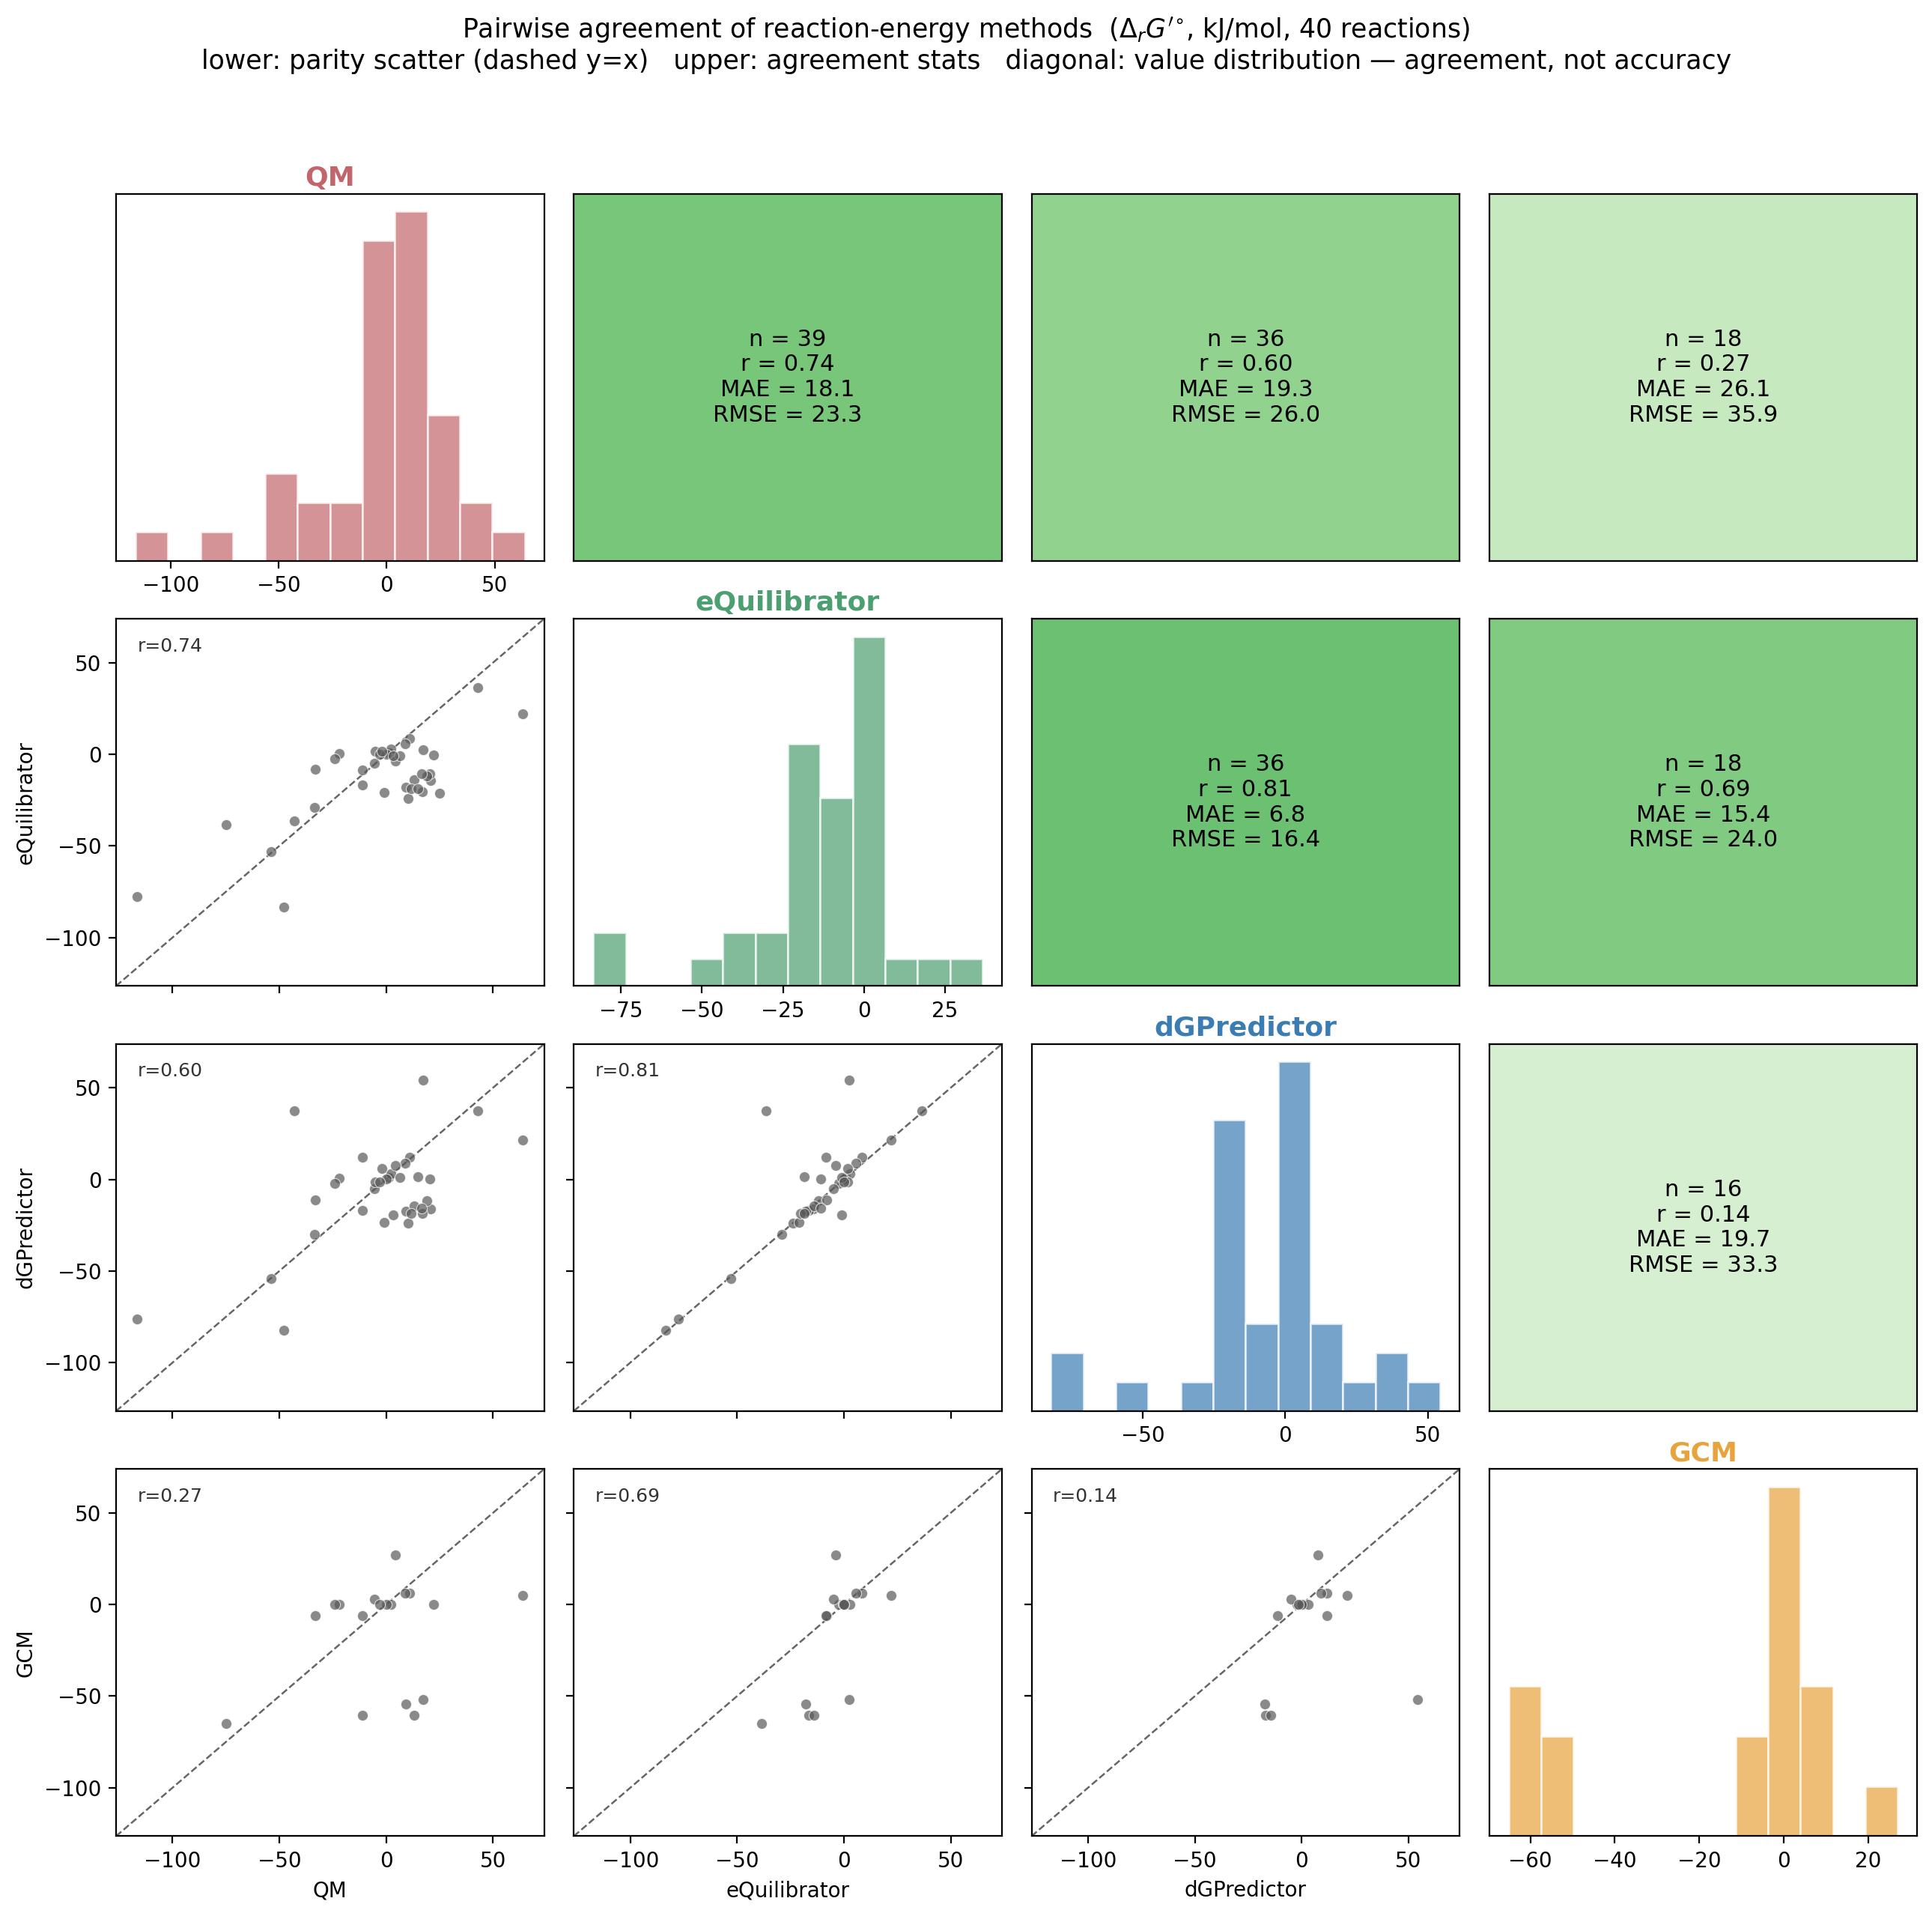
\includegraphics[height=0.78\textheight]{figures/method_pairplot.png}
      \end{center}
    \column{0.38\textwidth}
      \small
      Pairwise agreement over 40 reactions (agreement, \emph{not} accuracy):
      \begin{itemize}
        \item eQuilibrator$\leftrightarrow$dGPredictor agree best ($r=0.81$,
              MAE 6.8) — same data lineage.
        \item QM correlates with all three ($r=0.6$--$0.74$) but with a wide
              MAE ($\sim$18--26) — an \emph{independent} axis.
        \item GCM (GroupContribution) is the weakest ($r\!\le\!0.27$ vs.\ QM),
              and it is what dGPredictor shares a basis with.
      \end{itemize}
  \end{columns}
\end{frame}

\begin{frame}{The decisive negative result — why no correction rescues it}
  \begin{columns}[T]
    \column{0.5\textwidth}
      \textbf{Per-species anchoring is dead}\\[0.2em]
      Compound-grouped cross-validation on per-species offsets:
      \[
        R^2 = \lose{0.177}\quad(\text{in-sample }0.769)
      \]
      To tie predict-zero needs $R^2\!\approx\!0.89$; to match eQuilibrator
      $\approx\!0.97$. This rules out \emph{every} anchoring scheme at once
      ($\mu_H$, cofactor $E'^\circ$, anion-site corrections, reference-compound
      reformulation). The error is not in that subspace.
    \column{0.5\textwidth}
      \textbf{Mechanisms eliminated}\\[0.2em]
      \footnotesize
      \begin{tabular}{@{}ll@{}}
        \toprule
        mechanism & verdict \\
        \midrule
        electronic structure & \no\ (DFT worse) \\
        MLIP architecture     & \no\ ($r=0.98$) \\
        conformer sampling    & \no\ (wrong sign) \\
        Alberty transform     & \yes\ passes \\
        bond-graph artifact   & \no\ (0 changed) \\
        protonation state     & \yes\ correct \\
        Mg$^{2+}$ speciation  & \no\ ($+0.3\kj$ net) \\
        \bottomrule
      \end{tabular}
      \normalsize\\[0.4em]
      Diagnosis is \textbf{solid}; every candidate correction was
      \textbf{rejected} on its own test.
  \end{columns}
\end{frame}

% =====================================================================
\section{A learned component-contribution model}
% =====================================================================

\begin{frame}{``dGPredictor done right'' — a GNN, and an honest test}
  \begin{columns}[T]
    \column{0.5\textwidth}
      \textbf{The idea}\\[0.2em]
      Replace the linear group-contribution \emph{lookup table} with a
      message-passing \textbf{GNN} that maps each compound's graph to a scalar
      formation energy $f$; a reaction is the stoichiometric difference
      \[
        \Delta_r G'^{\circ} \;=\; \mathbf{S}\,f ,\qquad f=\text{GNN(compound)} .
      \]
      Trained on reaction \dg\ \emph{only} (no per-compound labels).
      \textbf{Sum readout} (energy is extensive) $+$ \textbf{QC injected as
      features} (xtb Mulliken charges, HOMO/LUMO, CPCM-X solvation) $+$
      \textbf{$\Delta$-learning} on the group prior.
    \column{0.5\textwidth}
      \textbf{Why it might beat the incumbents}
      \begin{itemize}
        \item No \emph{coverage cliff}: a GNN interpolates in representation
              space instead of failing on a missing group.
        \item Nonlinear group interactions $+$ QC physics the linear table
              cannot see.
      \end{itemize}
      \vspace{0.3em}
      \begin{alertblock}{The discipline that matters}
        Every number below is \textbf{held-out} cross-validation. The
        incumbents' famous 3.0 is \textbf{in-sample} — they were trained on
        these reactions.
      \end{alertblock}
  \end{columns}
\end{frame}

\begin{frame}{Result: the model class is \emph{not} the bottleneck}
  \begin{columns}[T]
    \column{0.54\textwidth}
      \begin{center}\small
      \begin{tabular}{@{}llrr@{}}
        \toprule
        model & eval & \shortstack{rand.\\CV} & \shortstack{cpd.-\\disj.} \\
        \midrule
        eQuilibrator / dGP    & \emph{in-sample} & \win{3.0} & --- \\
        \midrule
        predict-zero          & ---              & 9.7  & 10.4 \\
        linear group-CC       & held-out         & 6.6  & 8.7 \\
        GNN (graph only)      & held-out         & 7.0  & 8.9 \\
        \textbf{GNN $+$ QC $+$ $\Delta$} & held-out & \textbf{6.8} & \textbf{8.6} \\
        \bottomrule
      \end{tabular}
      \end{center}
      \footnotesize $n=367$ reactions, 453 compounds. Compound-disjoint $=$
      held-out \emph{compounds} (the extrapolation / coverage regime).
    \column{0.46\textwidth}
      \small
      \begin{itemize}
        \item Linear CC, GNN, GNN$+$QC and GNN$+\Delta$ all land within
              \textbf{$0.3\kj$} of each other.
        \item Random held-out $\sim$6.7 $\approx$ the \textbf{experimental noise
              floor} (TECRDB sd $\sim$6). Little room for \emph{any} model.
        \item Drive regularization down and in-sample hits 1.6 while held-out
              worsens — the overfitting made visible.
      \end{itemize}
      \begin{block}{Verdict}
        At $n=367$ the bottleneck is \textbf{data, not architecture}. A learned
        representation buys nothing over regularized group additivity.
      \end{block}
  \end{columns}
\end{frame}

\begin{frame}{But it is \emph{robust} — no blow-ups}
  \begin{center}
    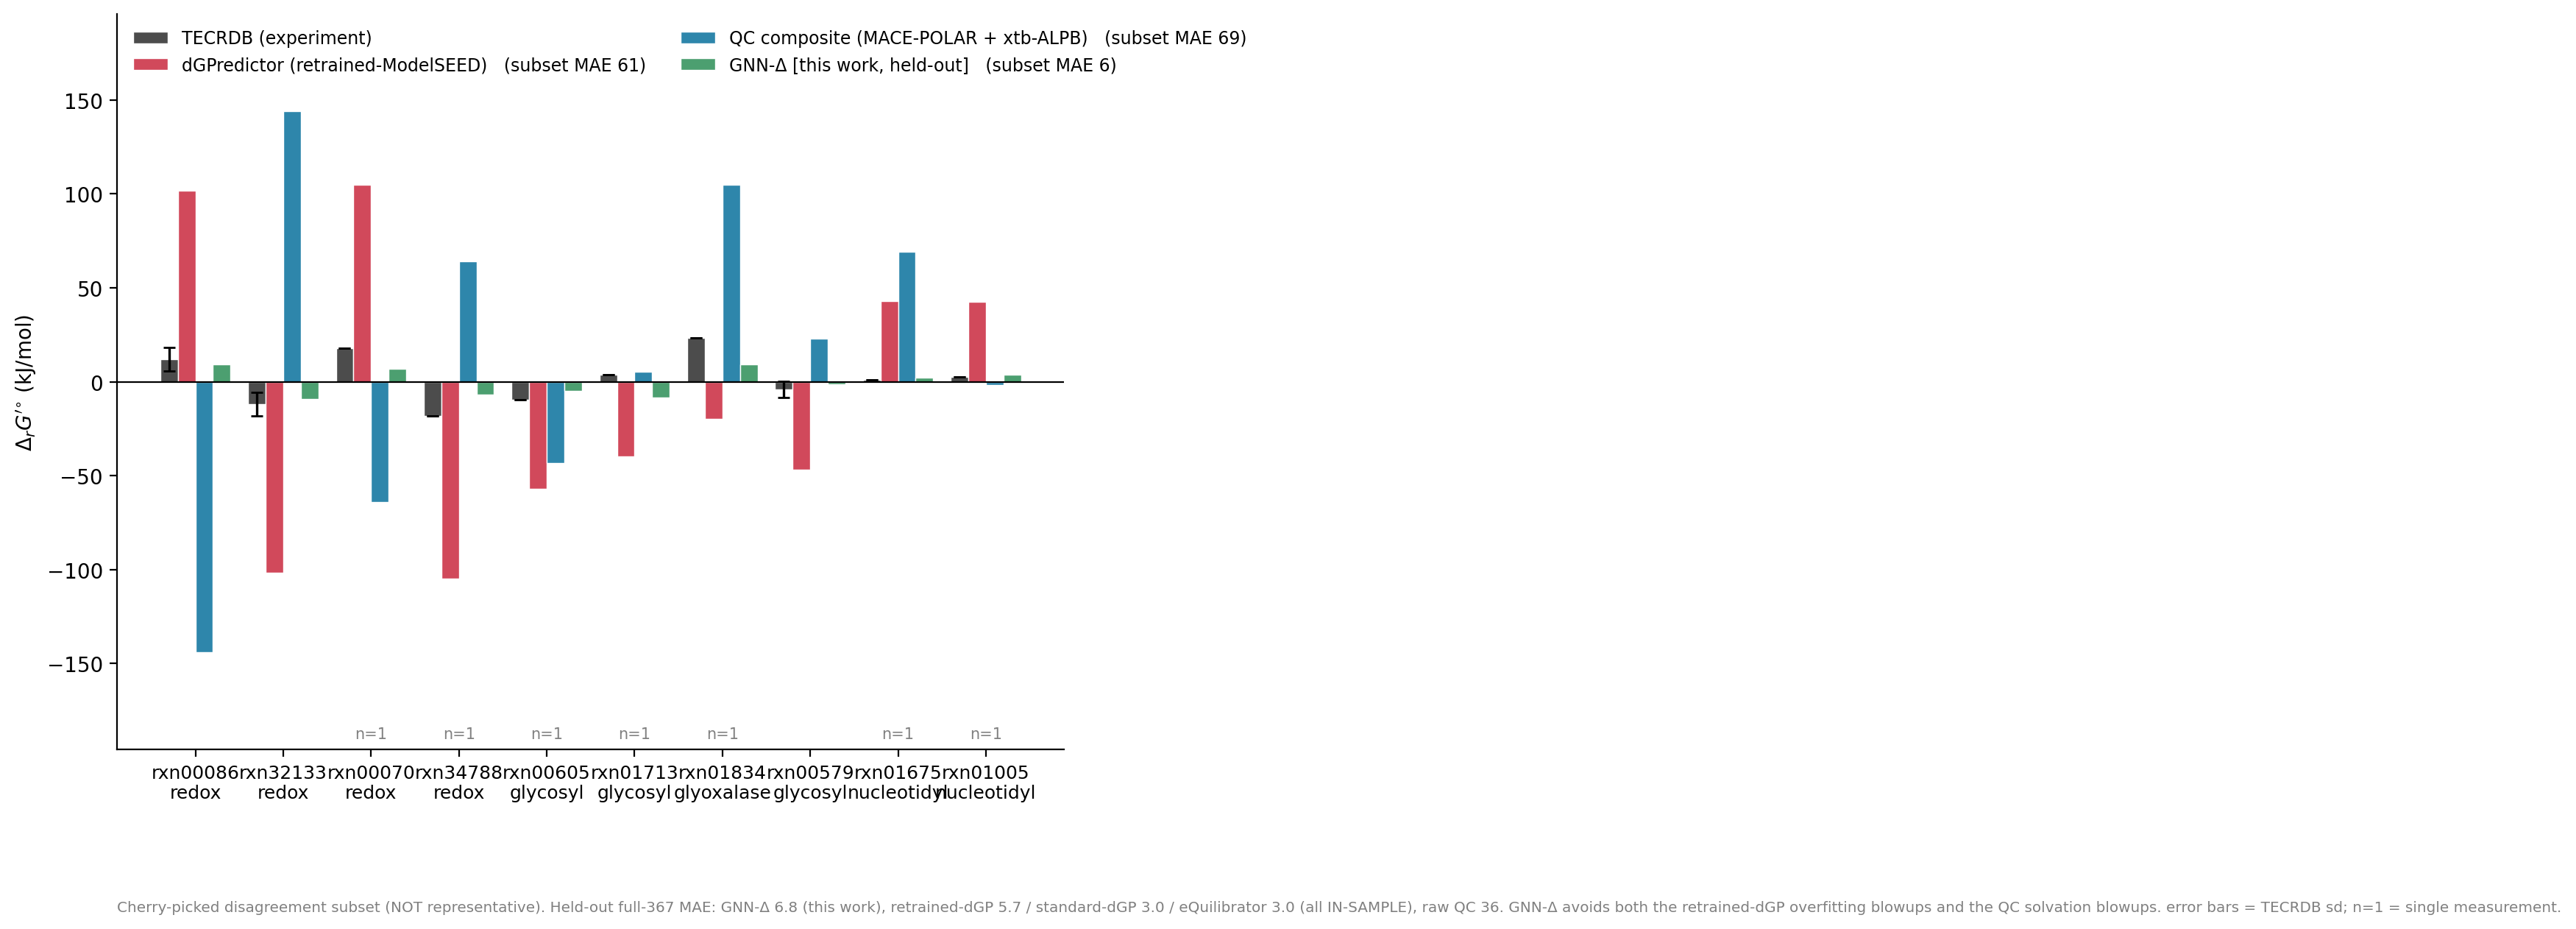
\includegraphics[height=0.70\textheight]{figures/qm_vs_dgpredictor_gnn.png}
  \end{center}
  \vspace{-0.4em}
  {\footnotesize On the cherry-picked hard subset the \textbf{GNN-$\Delta$}
  (\textcolor{good}{green}, held-out) tracks experiment — subset MAE \win{6} —
  while the retrained-dGP (\lose{red}, overfit blow-ups) and absolute QC
  (\textcolor{accent}{blue}, anion-solvation blow-ups) swing to $\pm$100.
  A well-regularized learned model dodges \emph{both} failure modes.}
\end{frame}

\begin{frame}{How QC can — and cannot — help}
  \begin{columns}[T]
    \column{0.5\textwidth}
      \textbf{Static QC features: marginal.} Per-compound charges/orbitals are
      redundant with group counts for the \emph{additive} part of formation
      energy; $n\!=\!367$ is too little to learn the nonadditive part they enable.
      \\[0.4em]
      \textbf{QC as a charge-gated prior: physics is right.} QC's absolute error
      $\sim$ Born $(z^2)$ anion under-solvation. A correction in
      $\Delta(\sum\nu z^2)$ \win{improves QC-alone} (9.4$\to$9.1) and
      \emph{transfers across compounds} — unlike group features.
    \column{0.5\textwidth}
      \begin{alertblock}{The catch}
        On TECRDB, QC still cannot beat group-additivity (9.1 vs 6.7) and adds
        nothing on top of it (6.94 vs 7.01). Every TECRDB reaction is
        group-coverable, so QC's real advantage is \textbf{invisible here}.
      \end{alertblock}
      \textbf{QC's payoff is coverage} — the $\sim$42\% of ModelSEED with no
      group decomposition — which has no experimental labels by construction.
      \\[0.3em]
      $\Rightarrow$ the lever is \textbf{training signal}: distil eQuilibrator
      over \textbf{56k} ModelSEED reactions into the GNN (in progress).
  \end{columns}
\end{frame}

% =====================================================================
\section{Where this leaves us}
% =====================================================================

\begin{frame}{Summary \& where QM should be pointed}
  \begin{columns}[T]
    \column{0.5\textwidth}
      \textbf{What we established}
      \begin{itemize}
        \item eQuilibrator solves the TECRDB disagreements; QM cannot beat it on
              aqueous polyanion chemistry.
        \item The limit is \textbf{continuum anion solvation}
              ($\sim$30\kj/reaction) — structural, reproduces the literature.
        \item Robust across electronic method, MLIP, CV, solvation swap and
              Mg$^{2+}$ bookkeeping.
        \item \win{The one real QM win}: on glutathione redox its magnitude
              independently excludes dGPredictor's $\pm$100, from zero training data.
      \end{itemize}
    \column{0.5\textwidth}
      \textbf{The open problem}
      \begin{itemize}
        \item QM is uniquely positioned where data-driven methods \emph{cannot}
              score: the 16\% of matched reactions eQuilibrator misses,
              stereochemistry (GCM is blind by construction), novel metabolites.
        \item But that regime has \textbf{no validation data by definition}.
        \item Next: design held-out compound classes / stereoisomer pairs
              \emph{before} more compute; long-term ceiling is explicit-solvent
              MD $+$ MLIP $+$ alchemical free energy.
      \end{itemize}
  \end{columns}
\end{frame}

\begin{frame}[standout]
  The physics cannot reach 5\kj\ on polyanions —\\
  but on the reactions that matter, it agrees with experiment\\
  \emph{for reasons the data-driven methods cannot claim}.
\end{frame}

\end{document}
